\documentclass[border=4pt]{standalone}

\usepackage{tikz}

\definecolor{otblue}{HTML}{0072B2}
\definecolor{otorange}{HTML}{E69F00}
\definecolor{otteal}{HTML}{009E73}
\definecolor{otpurple}{HTML}{CC79A7}
\definecolor{otgray}{HTML}{5A5A5A}

\begin{document}
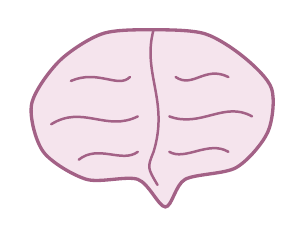
\begin{tikzpicture}[line width=0.9pt]
  \filldraw[draw=otpurple!80!black, fill=otpurple!20, line width=1.2pt] plot[smooth cycle] coordinates {(0,1.25) (0.65,1.2) (1.15,0.9) (1.5,0.5) (1.45,-0.05) (1.05,-0.5) (0.4,-0.65) (0.15,-1) (-0.2,-0.65) (-0.85,-0.65) (-1.4,-0.3) (-1.55,0.3) (-1.2,0.85) (-0.65,1.2)};
  \draw[otpurple!80!black, line cap=round] (0,1.25) .. controls (-0.15,0.7) and (0.2,0.35) .. (0,-0.3) .. controls (-0.08,-0.5) .. (0.05,-0.72);
  \draw[otpurple!80!black, line cap=round] (-1.05,0.6) .. controls (-0.7,0.75) and (-0.45,0.5) .. (-0.3,0.65);
  \draw[otpurple!80!black, line cap=round] (-1.3,0.05) .. controls (-0.9,0.3) and (-0.6,-0.05) .. (-0.2,0.15);
  \draw[otpurple!80!black, line cap=round] (-0.95,-0.4) .. controls (-0.7,-0.2) and (-0.4,-0.45) .. (-0.2,-0.3);
  \draw[otpurple!80!black, line cap=round] (0.95,0.65) .. controls (0.65,0.8) and (0.5,0.5) .. (0.28,0.65);
  \draw[otpurple!80!black, line cap=round] (1.25,0.15) .. controls (0.9,0.35) and (0.6,0) .. (0.2,0.15);
  \draw[otpurple!80!black, line cap=round] (0.95,-0.3) .. controls (0.7,-0.15) and (0.4,-0.42) .. (0.2,-0.3);
\end{tikzpicture}
\end{document}
